% results_retention.tex
\subsection{Factor Retention}

With no respondents to permute, \texttt{sfa\_parallel()} adapts
parallel analysis \citep{horn-1965}, retaining factors above the 95th
percentile of random-embedding null eigenvalues:

{\scriptsize
\begin{verbatim}
> pa <- sfa_parallel(sim_mcp, E8)
> pa
Embedding-adapted parallel analysis
  Suggested factors: 5
  Embedding dimension: 4096
  Iterations: 100
  Percentile: 95
\end{verbatim}
}

\texttt{sfa\_nfactors()} adds four criteria: eigenvalues greater than
one \citep{kaiser-1960}, the empirical Kaiser criterion, whose reference
eigenvalues correct for the variance preceding factors already absorbed
\citep{braeken-vanassen-2017}, TEFI \citep[following][]{golino-2026}, and
EGA, validated for embeddings by \citet{garrido-etal-2025}:

{\scriptsize
\begin{verbatim}
> nf <- sfa_nfactors(sim_mcp, embeddings = E8,
+                    methods = c("parallel", "kaiser", "TEFI", "EGA", "EKC"))
> nf
Factor retention analysis (embedding-adapted)

  Method       n_factors
  parallel     5
  kaiser       6
  TEFI         2
  EGA          5
  EKC          6
  ------------------------
  Consensus    5

Eigenvalues: 29.63   1.92   1.74   1.48   1.27   1.01   0.93   0.88   0.78   0.70  ...
\end{verbatim}
}

Parallel analysis and EGA indicated \valPaKWord{} factors, Kaiser \valKaiserKWord, the
empirical Kaiser criterion \valEkcKWord, TEFI
\valTefiKWord. The consensus of \valConsensusKWord{} matches the theoretical Big Five, and the
dominant first eigenvalue (\valEigFirst), the general positivity of embedding
similarities, precedes a shallow elbow (Figure~\ref{fig:scree}).

\begin{figure}[H]
\centering
\captionsetup{justification=raggedright,singlelinecheck=false}
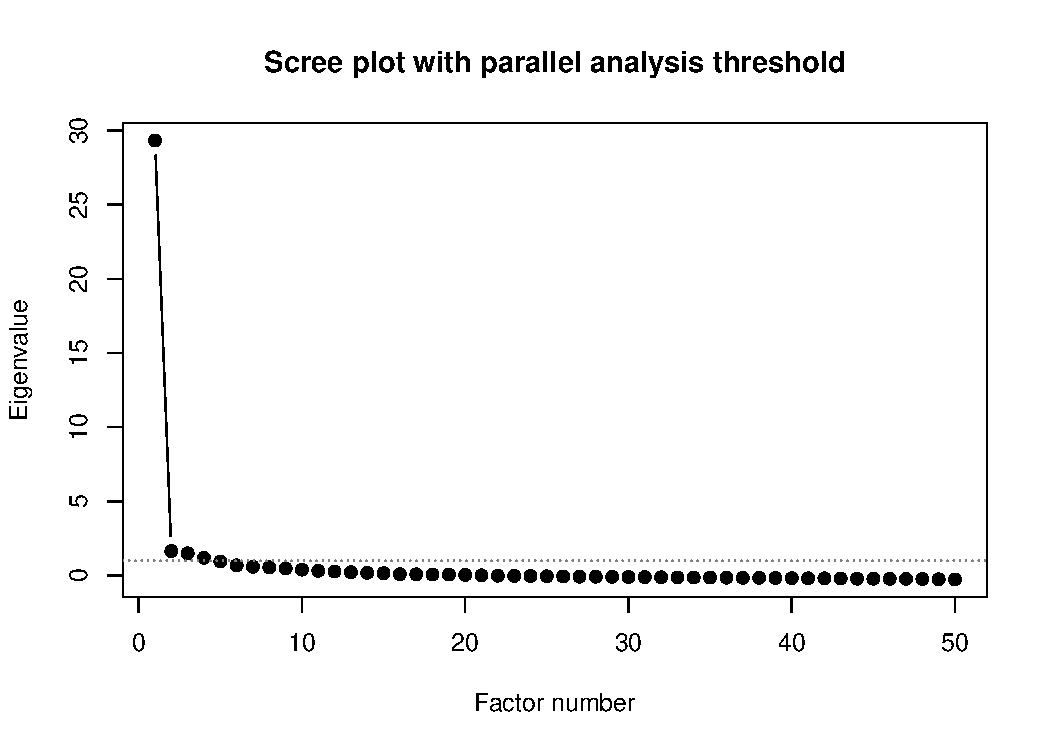
\includegraphics[width=0.6\textwidth]{figures/scree.pdf}
\caption{Scree plot of the mean-centered Pearson similarity matrix with the
embedding-adapted parallel-analysis threshold (dotted line), produced by
\texttt{plot(fit, type = "scree")}. The first eigenvalue (\valEigFirst) dwarfs the
rest, and \valPaKWord{} eigenvalues clear the parallel-analysis threshold.}
\label{fig:scree}
\end{figure}

A second question is embedding-specific: how many of the 4{,}096
coordinates carry structural signal? \texttt{sfa\_dimselect()} adapts
the embedding-depth optimization of \citet{golino-2026}, scoring swept
truncations by structural recovery (NMI) weighted against entropy fit
(TEFI):

{\scriptsize
\begin{verbatim}
> ds <- sfa_dimselect(E8, factors = big5$factors,
+                     encoding = "mean_centered_pearson")
> ds
EGA-based embedding-dimension selection
  Method: EGA depth optimization (adapts Golino 2026)
  Full embedding dim: 4096
  Depths evaluated:   148 (range 3-4096)
  Criterion:          0.70*NMI - 0.30*TEFI (normalized)
  Optimal depth:      1431 of 4096 coordinates
    at optimum: n_dim=5  NMI=0.704  TEFI=-23.291
> cat("sfa_dimselect elapsed:", round(t_ds["elapsed"], 1), "s\n")
sfa_dimselect elapsed: 28 s
\end{verbatim}
}

The optimum (roughly the first third, \valDepthOpt{} of \valDepthFull
coordinates) recovered \valDepthNDimWord{} EGA dimensions (NMI = \valDepthNmi), the
\valDepthNDimWord-factor answer by a different route. The \valDepthEval-depth sweep took
\valTimeDimselect~s.
